
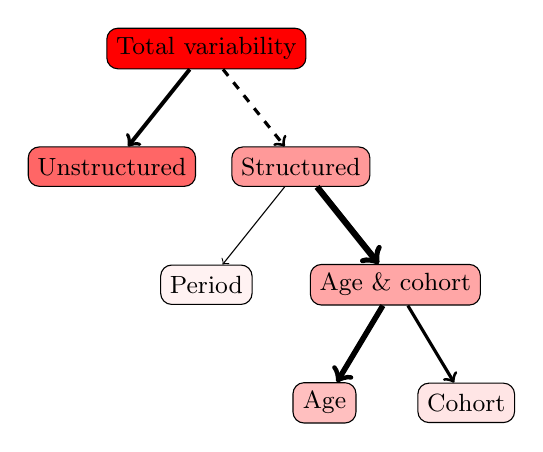
\begin{tikzpicture}[
    rounded corners,
    minimum height = 0.5cm, 
    minimum width = 0.8cm
]
\node[draw] (top) [fill = red!100] {{\color{black}\small Total variability}};
\node[draw] (gen) [below of = top, xshift = 1.2cm, yshift = -0.5cm, fill = red!40] {\small Structured};
\node[draw] (env) [below of = top, xshift = -1.2cm, yshift = -0.5cm, fill = red!60] {\small Unstructured};
\node[draw] (add) [below of = gen, xshift = -1.2cm, yshift = -0.5cm, fill = red!5] {\small Period};
\node[draw] (nonadd) [below of = gen, xshift = 1.2cm, yshift = -0.5cm, fill = red!35] {\small Age \& cohort};
\node[draw] (dom) [below of = nonadd, xshift = -0.9cm, yshift = -0.5cm, fill = red!25] {\small Age};
\node[draw] (epi) [below of = nonadd, xshift = 0.9cm, yshift = -0.5cm, fill = red!10] {\small Cohort};
% arrows
\path[->, every node/.style = {sloped, anchor = south, auto = false, anchor = mid, yshift = 0.15cm}]
(top) edge[line width = 0.5mm] node[] {} (env)
(top) edge[dashed, line width = 0.4mm] node[] {} (gen)
(gen) edge[] node[] {} (add)
(gen) edge[line width = 0.8mm] node[] {} (nonadd)
(nonadd) edge[line width = 0.7mm] node[] {} (dom)
(nonadd) edge[line width = 0.4mm] node[] {} (epi);

\end{tikzpicture}
